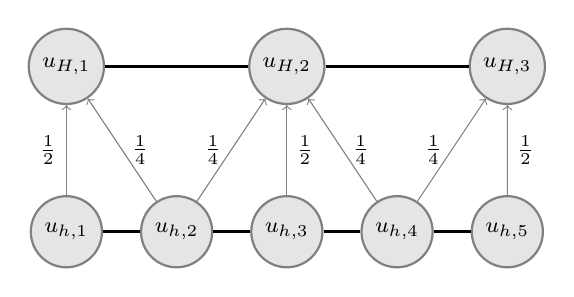
\begin{tikzpicture}[
node/.style={
  circle,
  draw=black!50,
  fill=black!10,
  thick,
  font=\footnotesize
},
scale=0.7,
arrownote/.style={black,font=\footnotesize}
]

\node (u1) at (0,3) [node] {$u_{H,1}$};
\node (u2) at (4,3) [node] {$u_{H,2}$};
\node (u3) at (8,3) [node] {$u_{H,3}$};

\node (u5) at (0,0) [node] {$u_{h,1}$};
\node (u6) at (2,0) [node] {$u_{h,2}$};
\node (u7) at (4,0) [node] {$u_{h,3}$};
\node (u8) at (6,0) [node] {$u_{h,4}$};
\node (u9) at (8,0) [node] {$u_{h,5}$};

\draw [very thick] (u1) -- (u2) --(u3);
\draw [very thick] (u5) --(u6) --(u7) --(u8) --(u9);

\draw [->,black!50] (u5) to node [arrownote,left] {$\frac{1}{2}$}  (u1);
\draw [->,black!50] (u6) to node [arrownote,right] {$\frac{1}{4}$} (u1);

\draw [->,black!50] (u6) to node [arrownote,left] {$\frac{1}{4}$} (u2);
\draw [->,black!50] (u7) to node [arrownote,right] {$\frac{1}{2}$} (u2);
\draw [->,black!50] (u8) to node [arrownote,right] {$\frac{1}{4}$} (u2);

\draw [->,black!50] (u8) to node [arrownote,left] {$\frac{1}{4}$} (u3);
\draw [->,black!50] (u9) to node [arrownote,right] {$\frac{1}{2}$} (u3);

\end{tikzpicture}
